\section{Kennlinien}

\subsection{Definitionen}
\begin{itemize}
	\item \textbf{Kalibrieren}\\
	Ermitteln der Beziehung zwischen Anzeigegröße bzw. Ausgangsgröße und dem wahren Wert der Messgröße
	\item \textbf{Eichen}\\
	Kalibrierung durch das Eichamt
	\item \textbf{Justierung bzw. Abgleich}\\
	Einstellen des Messgeräts um systematische Messfehler zu reduzieren, sodass die für die Anwendung erforderliche Genauigkeit erreicht werden kann. -> es wird in das Messgerät eingegriffen
\end{itemize}

\subsection{Reale und ideale Kennlinie}
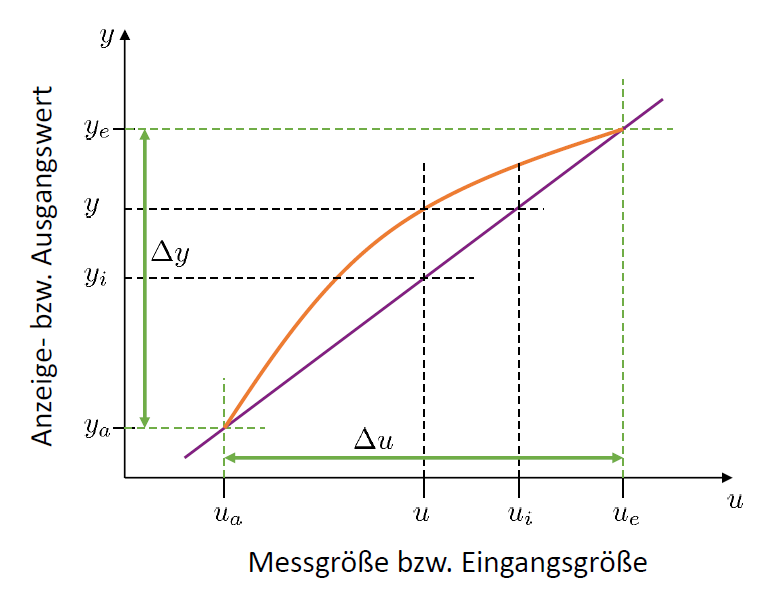
\includegraphics[width=\linewidth]{Figures/kennlinien/reale_ideale_kennlinie.png}
\begin{itemize}
	\item Messbereich: 		$\left[ u_a, u_e \right]; \Delta u = u_a - u_e$
	\item Anzeigebereich: 	$\left[ y_a, y_e \right]; \Delta y = y_a - u_e$
	\item Reale Kennlinie:	$y(u)$
	\item Empfindlichkeit:	$S(u) = \frac{dy(u)}{du}$
	\item Ideale Kennlinie:	$y_i = \frac{y_e - y_a}{u_e - u_a} \cdot (u - u_a) + y_a$
\end{itemize}

\subsection{Fixpunktjustierung}
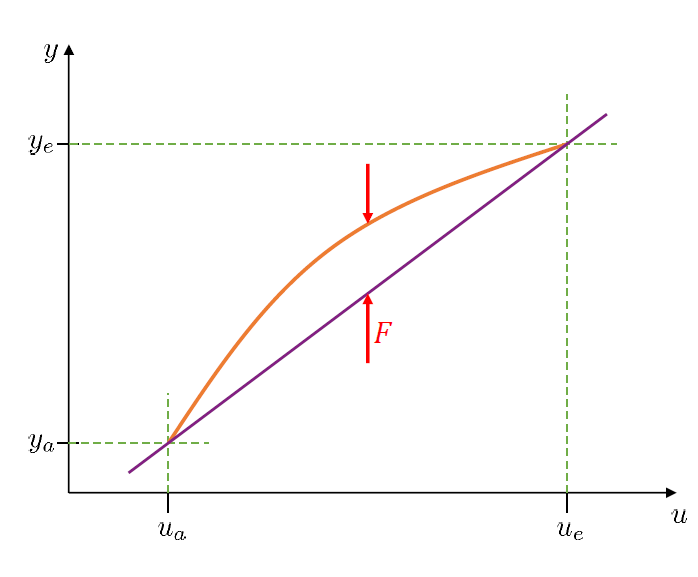
\includegraphics[width=\linewidth]{Figures/kennlinien/fixpunkt_justierung.png}
Justierung erfolgt, das ideale Kennlinie bie Normalbedingungen $\vec{z_0}$ durch den Anfangspunkt $(u_a, y_a)$ und den Endpunkt $(u_e, y_e)$ geht.\\
Der maximale Fehler F tritt an einer beliebigen Stelle zwischen Anfangs- und Endpunkt auf.
\[y_a = f(u_a, \vec{z_0}) \qquad y_e = f(u_e, \vec{z_0})\]
Am Anfangs- und Endpunkt ist Kennlinienfehler = 0. Bei Normalbedingungen ist der Offsetfehler definitionsgemäß = 0\\
\[ e(\vec{z_0}) = f(u_a, \vec{z_0}) - y_a = 0\]

\subsection{Toleranzbandjustierung}
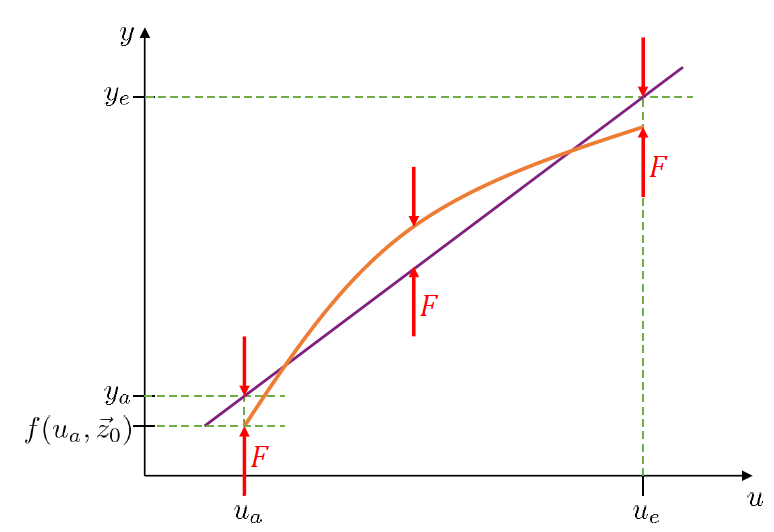
\includegraphics[width=\linewidth]{Figures/kennlinien/toleranzband_justierung.png}
Durch eine zusätzliche Verschiebung der idealen Kennlinie (Offset) kann der maximale Fehler der Fixpunktjustierung halbiert werden.\\
Der Offsetfehler entspricht dem maximalen Fehler.\\
Offsetfehler am Anfangspunkt:
\[ e(\vec{z_0}) = f(u_a, \vec{z_0}) - y_a \neq 0 \]
{\color{red} Achtung: überlegen wann sinnvoll!}

\subsection{Hysterese}
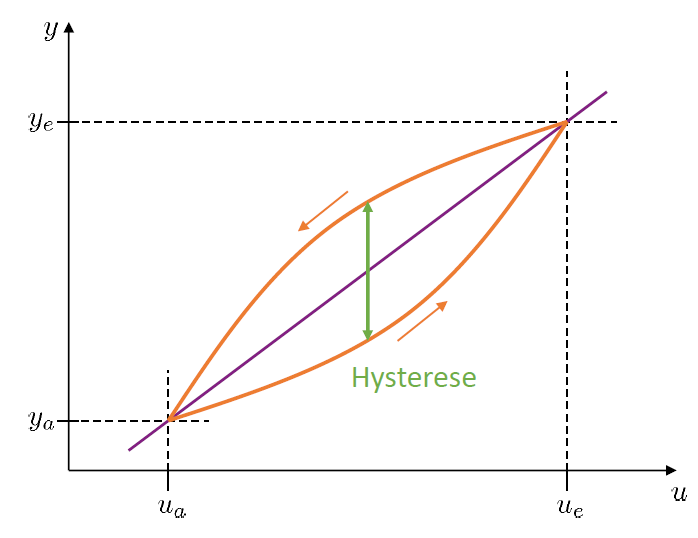
\includegraphics[width=\linewidth]{Figures/kennlinien/hysterese.png}
Hysterese kann durch sehr langsames Abfahren der Kennlinie in beide Richtungen ermittelt werden.\\
Als Hysterese wird die maximal auftretende Differenz verstanden.

\subsection{Umkehrspanne durch Hemmung}
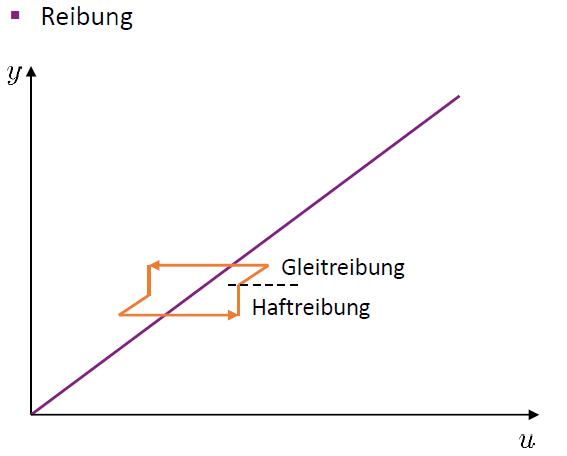
\includegraphics[width=\linewidth]{Figures/kennlinien/umkehrspanne_reibung.png}
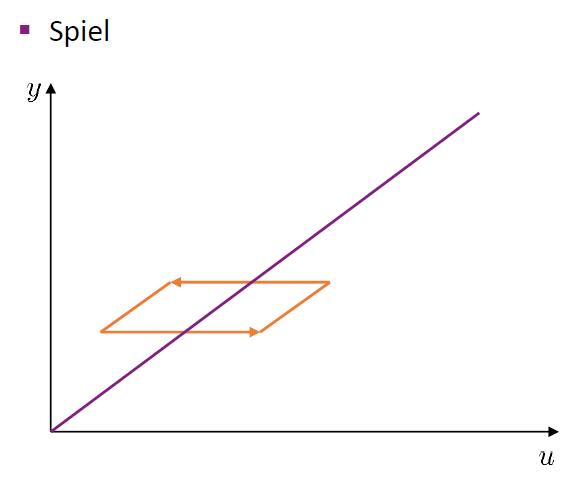
\includegraphics[width=\linewidth]{Figures/kennlinien/umkehrspanne_spiel.png}

\subsection{Mittlere Empfindlichkeit $\overline{S}$}
\fcolorbox{green}{white}{
	$\overline{S}(u,u_a,\vec{z_0}) = \frac{y - y_a}{u - u_a} = \frac{\Delta y}{\Delta u}$
}

\vspace{1ex} % Optional: Kleiner vertikaler Abstand zwischen den Boxen

\noindent
\fcolorbox{orange}{white}{
	$\begin{aligned}
		S(u,\vec{z}) &= \frac{df(u, \vec{z})}{du} \\[1ex]
		\overline{S}(u,u_a,\vec{z}) &= \frac{1}{\Delta u}\int_{u_a}^{u} S(u, \vec{z}) \, du
	\end{aligned}$
}

\vspace{2ex} % Abstand zur Grafik
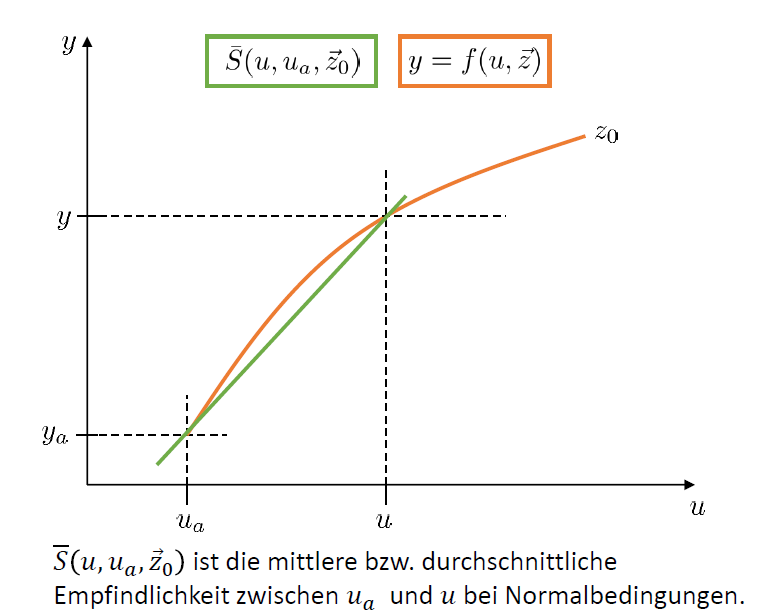
\includegraphics[width=\linewidth]{Figures/kennlinien/mittlere_empfindlichkeit.png}

\subsection{Relativer Kennlinienfehler}
Der relative Kennlinienfehler wird in dem die Empfindlichkeitsdifferenz auf die ideale Empfindlichkeit bezogen wird.
\[ F_r = \frac{\Delta S(u, \vec{z_0})}{S_i}\]
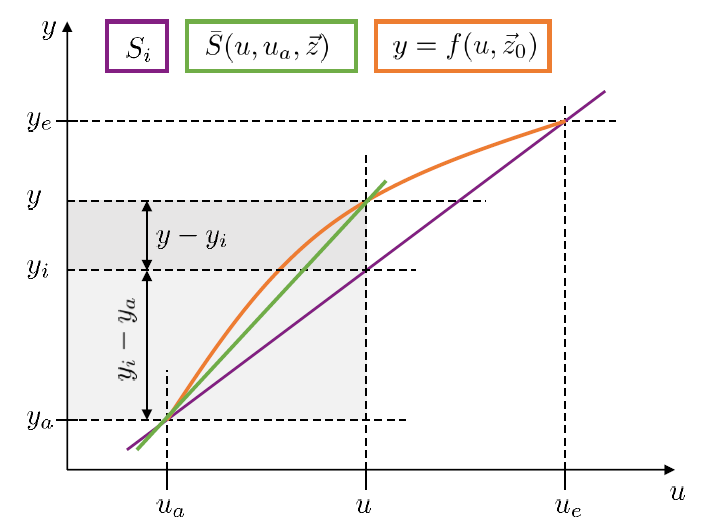
\includegraphics[width=\linewidth]{Figures/kennlinien/relativer_kennlinienfehler.png}
Zusammnhänge des rel. Kennlinienfehlers
\[\Delta y = \underbrace{S_i \cdot (1 + F_r)}_{\overline{S}(u, u_a, \vec{z}_0)} \cdot \Delta u\]
Die mittlere Steigung kann ungefähr ausgedrückt werden durch die Empfindlichkeit am Messanfang und die erste Ableitung der Empfindlichkeit.
\[ \overline{S}(u, u_a, \vec{z_0}) \approx S(u_a, \vec{z_0}) + \frac{1}{2!}S'(u_a, \vec{z_0}) \Delta u\]

\subsection{Methoden zur Linearisierung einer Kennlinie}
\subsubsection{Verringerung des Messbereichs}
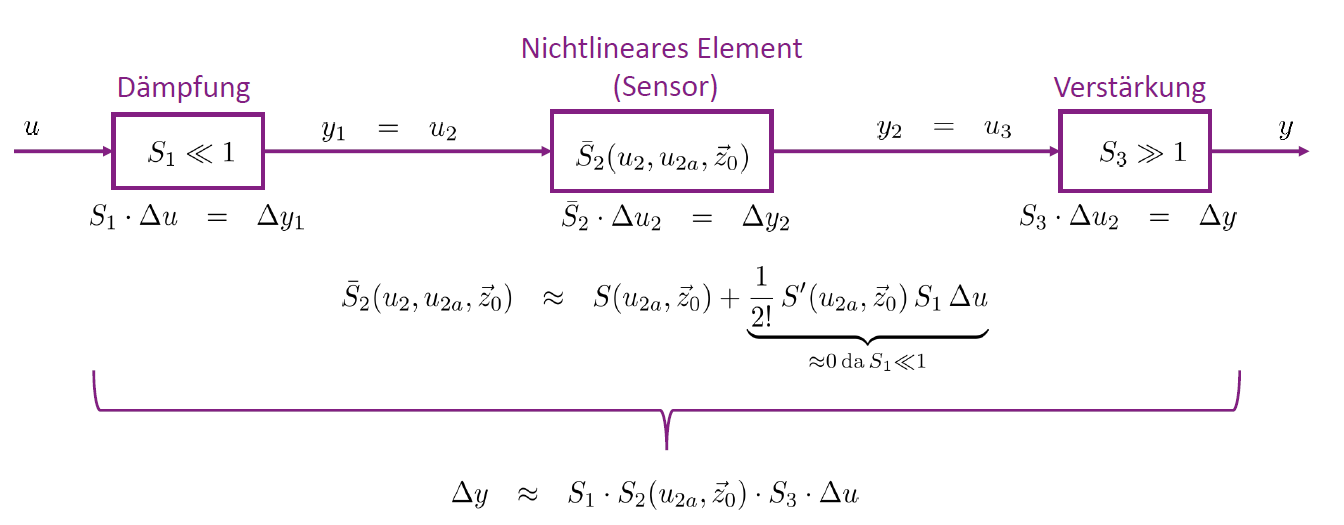
\includegraphics[width=\linewidth]{Figures/kennlinien/verringern_messbereich.png}
\[\Delta y\approx S_1 \cdot S_2(u_a, \vec{z_0}) \cdot S_3 \cdot \Delta u \]

\subsubsection{Nichtlineares Element zur Kompensation}
Approximation über konst. Steigung. Es muss die Umkehrfunktion zum Sensorelement gefunden und verwendet werden.\\
Beispiel Sensor quadriert, Kompensation zieht Wurzel\\
\vspace{2ex}
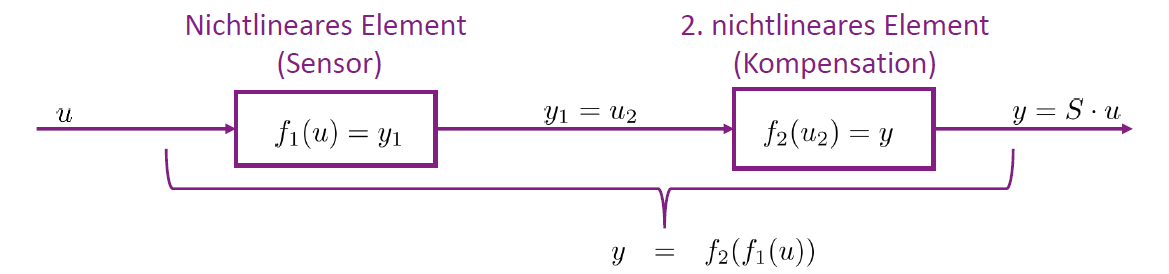
\includegraphics[width=\linewidth]{Figures/kennlinien/nichtlineares_element.png}

\begin{align*}
		y &= f_2(f_1(u)) \\[1.5ex]
		S &= \frac{dy}{du} = \frac{dy}{dy_1} \cdot \frac{dy_1}{du} = f_2' \cdot f_1' \stackrel{!}{=} \text{const.} \\[1.5ex]
		S' &= \frac{d^2y}{du^2} = f_2'' \cdot (f_1')^2 + f_2' \cdot f_1'' = S_2' \cdot S_1^2 + S_2 \cdot S_1' \stackrel{!}{=} 0
\end{align*}
	
\vspace{2ex}

\noindent
\fcolorbox{orange}{white}{$S_2'(f_1(u_a)) = -\frac{S_2(f_1(u_a)) \cdot S_1'(u_a)}{S_1^2(u_a)}$}
\hspace{1ex}
\fcolorbox{orange}{white}{$\dfrac{S_2'}{S_2} = -\dfrac{S_1'}{S_1^2}$}

\subsubsection{Differenzmethode}
Kann nur realisiert werden, wenn die Änderung in beide Richtungen möglich ist!\\
Es werden der gerade Anteil und der Offset unterdrückt.\\
Gerade und ungerader Anteil der Kennlinie um den Arbeitspunkt $u_0$
\[ g(\Delta u) = g_g(\Delta u) + g(\Delta u)\]
\[ g_g(\Delta u) = \frac{1}{2}(g(\Delta u) + g(-\Delta u))\]
\[ g_u(\Delta u) = \frac{1}{2}(g(\Delta u) - g(-\Delta u))\]
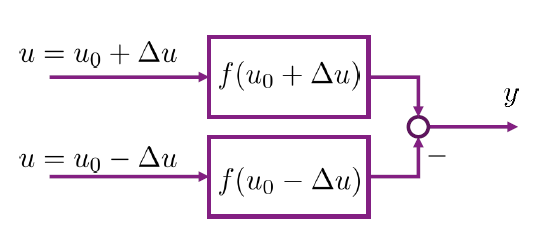
\includegraphics[width=\linewidth]{Figures/kennlinien/differenzmethode.png}
\[ y = g(\Delta u) - g(-\Delta u) = 2g_u(\Delta u)\]
\subsubsection{Gegenkopplung}
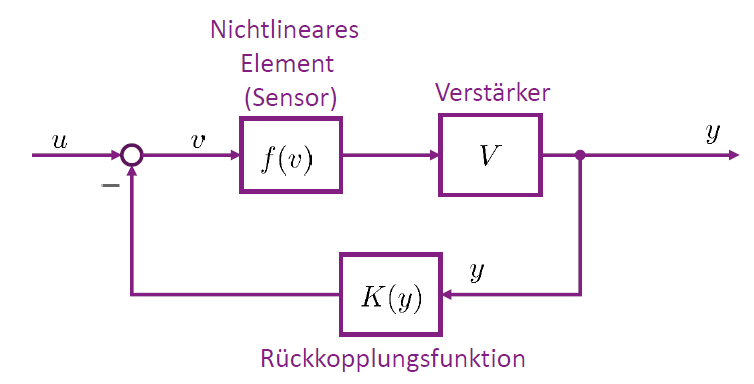
\includegraphics[width=\linewidth]{Figures/kennlinien/rueckkopplung.png}
\[ \underbrace{y = S_i \cdot V \cdot v \qquad v = u - K(y)}_{v = \frac{y}{S_i \cdot V} = u - K(y)}\]
\[ K(y) = u - \frac{y}{S_i \cdot V}\]
wenn V >> 1:
\[ K(y) \approx u\]
\begin{itemize}
	\item Allgemeiner Zusammenhang
	\[y_i = K^{-1}(u)\]
	\item Zusammenhang mit lin. Funktion K(y)
	\[ y_i = \frac{u}{K'}\]
	\item Relativer Kennlinienfehler
	\[ F_r = -\frac{1}{1 + S_i \cdot V \cdot K'}\]
	Mit ausreichender Verstärkung wird $F_r$ kleiner
\end{itemize}

\subsubsection{Wendepunkt}
Deformieren der Kennlinie, dass sich innerhalb des Messbereichs ein Wendepunkt befindet.\\
Damit kann die Abweichung von der idealen Kennlinie minimiert werden.\\
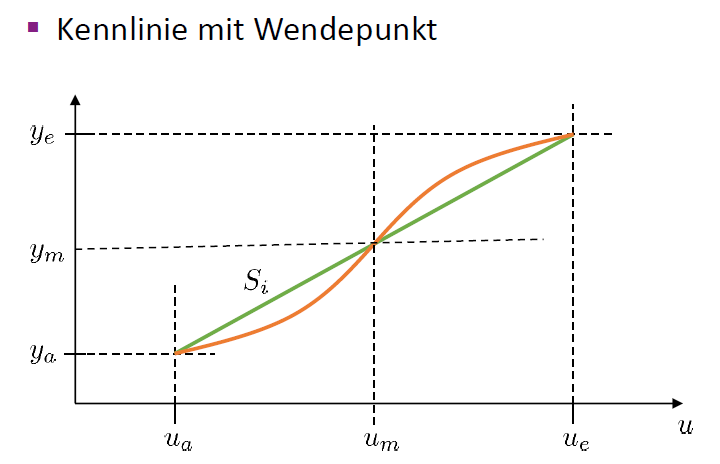
\includegraphics[width=\linewidth]{Figures/kennlinien/wendepunkt.png}
Steigungen von Bereich 1 und Bereich 2 gleichsetzen $\rightarrow$ Auflösen nach gesuchter Größe

\vspace{1ex}
\textbf{Linearisierung eines nichtlinearen Widerstands über einen Spannungsteiler:}
\[ R_0 = \frac{2 \cdot R_{\text{anfang}} \cdot R_{\text{ende}} - R_m \cdot (R_{\text{anfang}} + R_{\text{ende}})}{2 \cdot R_m - (R_{\text{anfang}} + R_{\text{ende}})} \]

\subsection{Fehlerursachen und Gegenmaßnahmen}
\subsubsection{Superponierende Fehler (Offset)}
\begin{itemize}
	\item Verschiebung der Messkennlinie.
	\item Fehlereinfluss überall gleich
	\item Empfindlichkeit ändert sich nicht
\end{itemize}
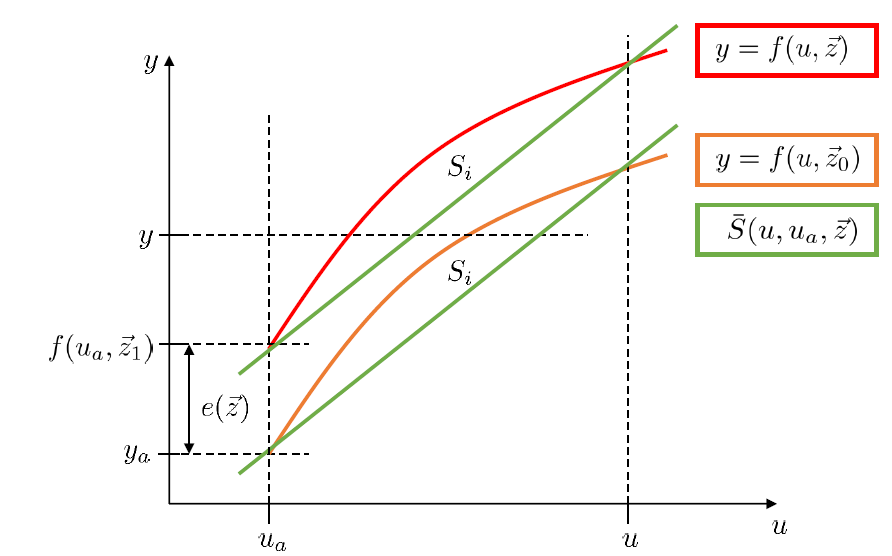
\includegraphics[width=\linewidth]{Figures/kennlinien/superponierende_fehler.png}
$\Rightarrow$ Eliminierung des Offsets durch Differenzmethode
\subsubsection{Deformierende Störgrößen}
\begin{itemize}
	\item Offsetfehler ändert sich nicht
	\item Steigung bzw. Empfindlichkeit ändert sich additiv
\end{itemize}
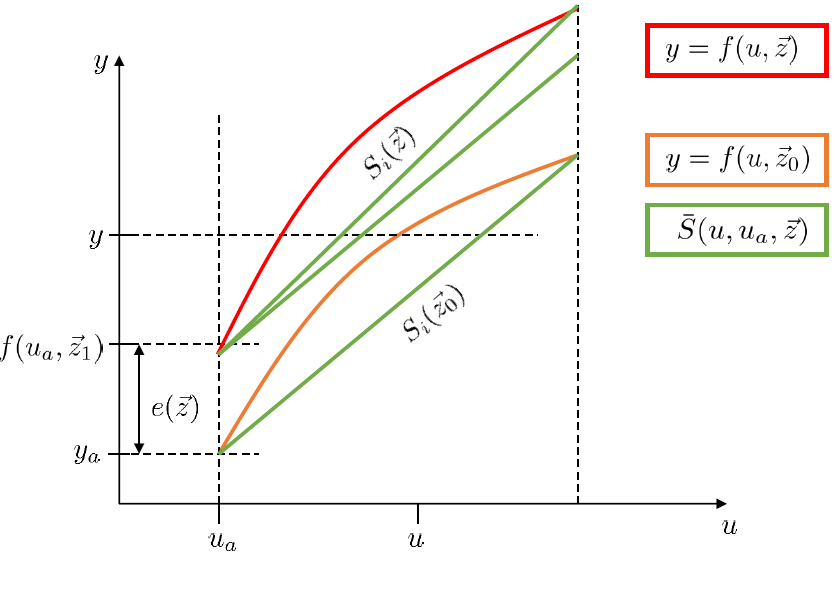
\includegraphics[width=\linewidth]{Figures/kennlinien/deformierende_stoergroeßen.png}
$\Rightarrow$ Eliminierung der deformierenden Störgrößen durch Gegenkopplung

\subsubsection{Superponierende Störgrößen bei Gegenkopplung}
\begin{itemize}
	\item lineare Rückkopplung
	\[ y = \frac{S_i \cdot V \cdot u}{1 + S_i \cdot V \cdot K'} + \frac{V \cdot z}{1 + S_i \cdot V \cdot K'}\]
	\item beliebige Rückkopplung und sehr große Verstärkung V
	\[ y \approx K^{-1}(u) \qquad \text{ohne Störung}\]
	\[ y \approx K^{-1}(u + \frac{z}{S_i}) \qquad \text{mit Störung}\]
	\item Die superponierende Störgröße bleibt grundsätzlich erhalten und kann durch die Gegenkopplung nicht eliminiert werden. Vorteilhaft ist eventuell, falls der Sensor eine sehr große Empfindlichkeit $S_i$ besitzt.
\end{itemize}
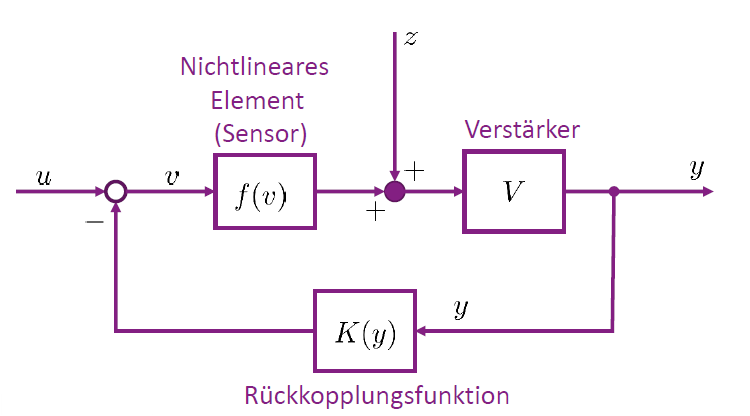
\includegraphics[width=\linewidth]{Figures/kennlinien/störgrößen_gegenkopplung.png}

\subsubsection{Kompensation und Abschirmung}
\begin{itemize}
	\item Systematische bzw. bekannte Störeinflüsse\\
	$\rightarrow$ dominante und messbare Störgrößen deren Einfluss auf die Ausgangsgröße bekannt sind können in der Ausgangsgröße eliminiert werden
	\item Abschirmung\\
	$\rightarrow$ Messsystem wird von dominierenden Messgrößen befreit\\
	Beispiel: Temperaturstabilisierung
\end{itemize}

\subsubsection{Additive (superponierende) Fehler in einer Messkette}
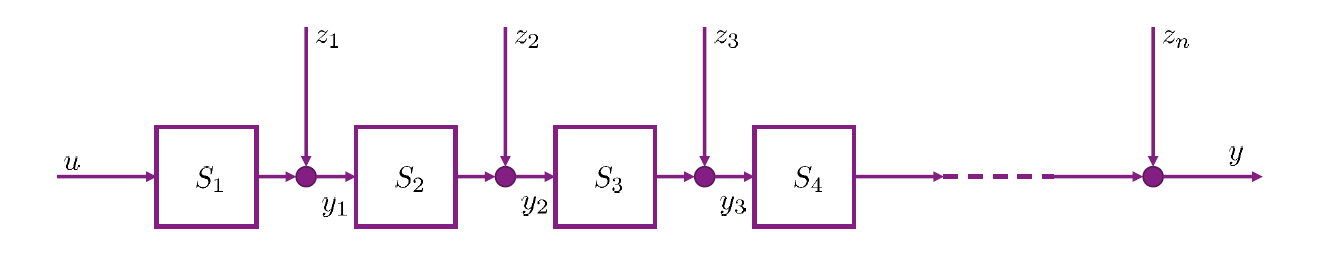
\includegraphics[width=\linewidth]{Figures/kennlinien/additive_superponierende_fehler.png}
pro Stufe gilt: \[ y_i = S_i \cdot y_{i-1} + z_i\]

\subsubsection{Rückwirkung}
Während des Messens beeinflusst das Messgerät die Messgröße